\documentclass[10pt]{beamer}

\usepackage{amssymb,amsthm}% http://ctan.org/pkg/amssymb
\newtheorem{proposition}{Proposition}
\setbeamertemplate{theorems}[numbered]
\usecolortheme[RGB={100,0,0}]{structure}
\setbeamercolor{block title}{use=structure,fg=white,bg=structure.fg!75!black}
\setbeamercolor{block body}{parent=normal text,use=block title,bg=block title.bg!10!bg}

\setbeamertemplate{footline}[frame number]

\usepackage{amsmath}
\DeclareMathOperator*{\argmax}{argmax}
\DeclareMathOperator*{\argmin}{argmin}

\usepackage{natbib}
\bibliographystyle{aea}

\usepackage{xcolor}
\usepackage{graphicx}
\usepackage{amsmath}
\usepackage{numprint}
\npdecimalsign{.}
\nprounddigits{3}
\usepackage{colortbl}
\usepackage{appendixnumberbeamer}
\usepackage{subfigure}
\usepackage{comment}

\usepackage{hyperref}
\usepackage{caption}
\setbeamerfont{caption}{size=\small}
\usetheme{Singapore}
\usecolortheme{beaver}

% for adding regression tables
\usepackage{dcolumn}
% column to line up decimals
\usepackage{booktabs,caption}
\captionsetup[table]{name=Table}
\setlength{\abovecaptionskip}{-1pt}
\setlength{\belowcaptionskip}{-1.5pt}
\usepackage[flushleft]{threeparttable} 
% The above two allow that last line with the dagger as a bottom note.

\usepackage{xcolor}
\definecolor{underbrace}{RGB}{30,199,166}
\newcommand{\textfrac}[1]{
  \begin{tabular}{@{}l@{}}#1\end{tabular}
}
\usepackage{tcolorbox}
\setbeamertemplate{caption}[numbered]

\title[ERPT]{Exchange Rate Pass-Through and Importers' Credit Constraints: Evidence From China}

\author[Li \& Lu]{Yao Amber Li\inst{*} \and Lingfei Lu\inst{*} \and Tengyu Zhao\inst{*}}

\institute[2024]{\inst{*} \small The Hong Kong University of Science and Technology}

\date{JIMF Special Issue Conference \\ Global Economic Order and Regional Cooperation:\\ Opportunities and Challenges \\ \vspace{3mm} Shanghai, China \\ \vspace{3mm} June 30, 2024 }


\begin{document}
	
\begin{frame}
    \maketitle
    \centering
\end{frame}

\AtBeginSection[]
{
    \begin{frame}{Outline}
    \transfade
    \tableofcontents[sectionstyle=show/shaded,subsectionstyle=show/shaded/hide]
    \addtocounter{framenumber}{-1}
    \end{frame}
}

\section{Introduction}

\begin{frame}[label=motivation1]{Motivations}
    \begin{itemize}
	\item Exchange rate shock is a key factor affecting international trade price fluctuations.
        \bigskip
	\item The impact of exchange rate changes on prices denominated in buyers' and sellers' currencies may be different, which leads to the studies on exchange rate pass-through.
        \bigskip
        \item Exchange rate pass-through (ERPT) is defined as \textbf{the elasticity of local price changes to exchange rate changes}.\hyperlink{example_ERPT}{\beamergotobutton{Example}}
        \bigskip
	\item Understanding the pattern of ERPT has important implications for formulating macro policies, including monetary policy, inflation targeting, and the balance of payments.
    \end{itemize}
    
\end{frame}

\begin{frame}[label=motivation2]{Motivations}
    \begin{itemize}
        \item Import sourcing is crucial for firm performance and aggregate welfare, while less is known about import-side (or buyer-side) ERPT with firm-level evidence. 
        \bigskip
	\item The credit constraints could be an important factor for significant firm heterogeneity in ERPT.
        \bigskip
	\item It remains an open question whether \textbf{importers under financial constraints will behave differently} in price setting during exchange rate fluctuations compared to those less constrained.
    \end{itemize}
\end{frame}

\begin{frame}{Research Questions}
    \begin{enumerate}
        \item What is the degree of ERPT among importers in China? 
        \bigskip
	\item How do credit constraints affect the importers' ERPT? 
        \bigskip
	\item What factors will enhance or mitigate this impact of credit constraints on import ERPT?
    \end{enumerate}
\end{frame}

\begin{frame}{What We Find}
Using Chinese customs transaction records and firm-level data:	
\medskip
    \begin{enumerate}
	\item The baseline import ERPT in China is around 73\%.
        \medskip
	\item Importers with tighter financial constraints have more complete ERPT.
        \medskip
	\item Importers with a higher degree of sourcing diversity (e.g., those who import a certain product from more sources) have a less complete ERPT and are less affected by credit constraints.
    \end{enumerate}	
\end{frame}

\begin{frame}{Contribution: Incomplete Exchange Rate Pass-Through}
    \begin{itemize}
	\item We contribute to the literature of exchange rate disconnect, particularly on firm-level evidence of \textbf{incomplete ERPT}.
        \medskip
	\item Related literature:
	\begin{itemize}
		\item \cite{bmm2012} (BMM): micro-level evidence of firm heterogeneity in response to real exchange rate shocks.
		\item \cite{aik2014} (AIK): firms with higher import intensity and larger market share have lower ERPT.
		\item More works: \cite{lmx2015}, \cite{chen2016}, \cite{garetto2016}, \cite{auer2016}, \cite{devereux2017}, etc.
	\end{itemize}
        \medskip
	\item Our contribution is to examine how \textbf{import} ERPT is affected by \textbf{credit constraints} using highly disaggregated data, particularly important for emerging markets with immature financial markets.
	\end{itemize}
\end{frame}

\begin{frame}{Contribution: Credit Constraints and Trade}
    \begin{itemize}
	\item This paper adds to the literature related to \textbf{the effects of credit constraints on firms' trade behaviors}.
        \medskip
        \item E.g.: \cite{manova2013}, \cite{chaney2016}, \cite{manova-wei-zhang2015}, \cite{fan-lai-li2015}.
        \item A few studies discuss how credit constraints affect firms' \textbf{export} responses to exchange rate fluctuations.
        \begin{itemize}
            \item \cite{strasser2013} shows that financially constrained firms tend to pass more exchange rate shocks to export prices.
		\item \cite{dai2021} and \cite{xu-guo2021} explore the export response to exchange rate shock under credit constraints. 
        \end{itemize}
        \medskip
    \item We contribute by uncovering the role of credit constraints in affecting \textbf{import EPRT} and showing how sourcing capacity (diversity) helps alleviate such impacts. 
	%\item We contribute to this literature by \textcolor{blue}{focusing on how importers behave under varying degrees of credit constraints and comparing their heterogeneous capacity to absorb exchange rate shocks}. 
    \end{itemize}	
\end{frame}

\section{Data and Measurements}

\begin{frame}{Data: Exchange Rates and Macro Variables}
	\begin{itemize}
		\item The bilateral nominal exchange rate is defined as the number of home currency units that can purchase a unit of foreign currency.
		\item The CPI-based real exchange rate ($RER_{ct}$) is defined as:
		$$
		RER_{ct}=NER_{ct} \cdot \frac{CPI_{ct}}{CPI_{CHN,t}}.
		$$
		\item An increase in $RER_{ct}$ means a real depreciation of the Chinese RMB against the
		foreign country’s $c$ currency.
		\item We use the real GDP of trading partners computed with national accounts growth, $RGDP_{ct}$, as the control variable of foreign supplies.
	\end{itemize}
\end{frame}

\begin{frame}{Data: Exchange Rates Fluctuations}
    \begin{figure}[htbp]
	\centering
	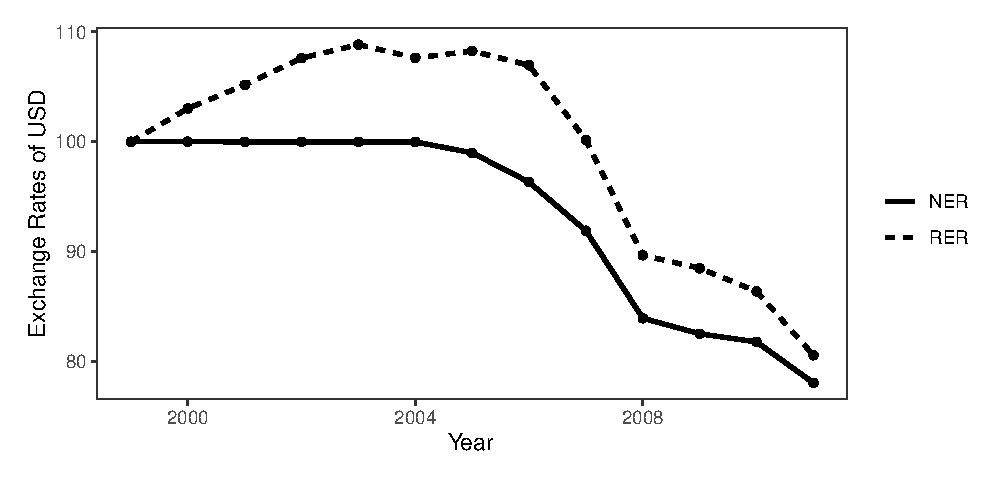
\includegraphics[width=0.65\columnwidth]{R/USD.eps}
        \label{fig.USD}
    \end{figure}
    \begin{figure}[htbp]
	\centering
	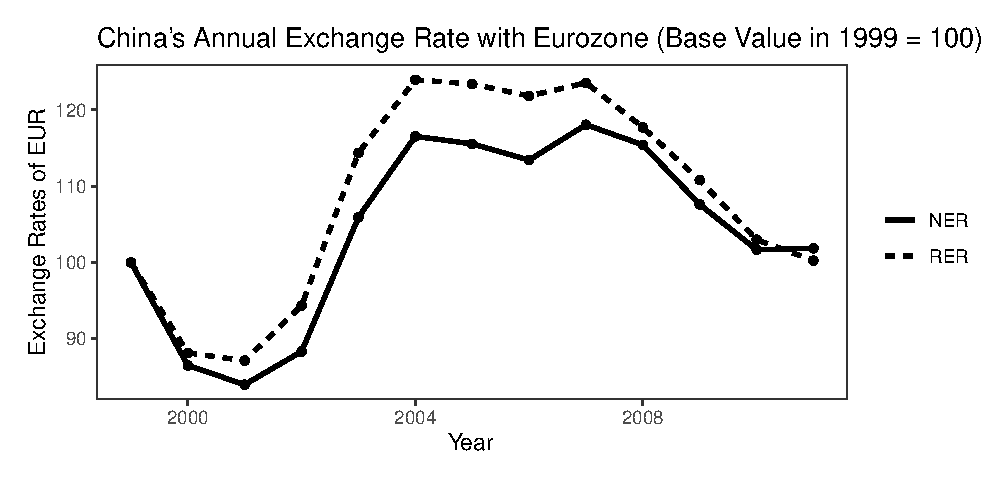
\includegraphics[width=0.65\columnwidth]{R/EUR.eps}
	\label{fig.EUR}
    \end{figure}
\end{frame}

\begin{frame}{Data: Firm-level and Customs data}
    \begin{itemize}
	\item Annual surveys of industrial enterprises from the National Bureau of Statistics of China
	\begin{itemize}
		\item Sample: all state-owned enterprises and above-scale firms (sales $>$5 million RMB), 1999 to 2007 
            \item Information: balance sheet variables, sales, employment, etc.
	\end{itemize}
        \medskip
        \item China Customs Records (from the General Administration of Customs of China)
        \begin{itemize}
            \item Sample: all exporting firms (except whole-sellers) in 2000-2011; matched manufacturing firms in 2000-2007 (baseline).
            \item Information: import and export values, quantities, product names and codes, source and destination countries, and firm types
	\end{itemize}
    \end{itemize}
\end{frame}

\begin{frame}{Data: Summary Statistics}
    \begin{table}[htbp]
        \centering
	\caption{Summary statistics for customs and firm data}
	\label{tab.summary.sample}
	\resizebox{\textwidth}{!}{
	\begin{threeparttable}
	\begin{tabular}{lcccccc}
		\toprule
             & Mean & Median & {Std. Dev} & P10 & P90 & \#observations\\
            \midrule
		\textbf{Panel A: Firm information} &       &       &       &       &       &  \\
		Sales Income (in 1000 RMB)  & 81492 & 18164 & 737089 & 5465  & 114840 & 1,619,194\\
		Employment (persons) & 256 & 106   & 939 & 30    & 491 & 1,619,194\\
		Fixed Asset (in 1000 RMB)  & 27398 & 4025  & 311063 & 572   & 36586 & 1,619,194\\
		Operation Input (in 1000 RMB)  & 63645 & 14318 & 580861 & 4143  & 90624 & 1,619,194\\
		Current wage payable (in 1000 RMB)  & 3802 & 1144  & 29502 & 278   & 6404 & 1,619,194\\
		\midrule
		\multicolumn{2}{l}{\textbf{Panel B: Matched sample with customs data}}       &       &       &       &       &  \\
  		Annual Import Price Change   & -0.0851 & -0.0018 & 1.4129 & -1.3406 &  1.1411 & 1,478,176\\
            Value per Transaction (in 1000 USD)  & 1140.97 & 14.81 & 18807.06 & 0.34 & 689.87 & 1,478,176\\
            \# Sources per Firm-product  & 2.07 & 1 & 2.27 & 1 & 4 & 1,478,176\\
		Annual Export Price Change  & 0.0248 & 0.0056 & 0.7101 & -0.5251 & 0.5940 & 1,724,591\\
            Value per Transaction (in 1000 USD)  & 786.32 & 44.08 & 17472.43 & 1.92 & 850.69 & 1,724,591\\
            \# Destinations per Firm-product  & 9.56 & 5 & 10.94 & 1 & 24 & 1,724,591\\
		\bottomrule
	\end{tabular}
	\begin{tablenotes}
            \footnotesize
    	\item Notes: This table shows the summary statistics of some important variables in our major datasets. Panel A describes sales and costs information of Chinese manufacturing firms during 2000-2007. The observations in panel A are at the firm-year level. The money values in panel A are in thousands of RMB. Panel B describes the price change, the value per transaction, and the number of sources (destinations) from (to) which each firm imports (exports) a certain HS6 product for the matched sample. The observations in panel B are at the firm-product-country-year level. The money values in panel B are in thousands of USD.
        \end{tablenotes}
	\end{threeparttable}
        }
    \end{table}
\end{frame}

\begin{frame}{Measures of Credit Constraints}
	\begin{itemize}
		\item Following \cite{manova-wei-zhang2015} and \cite{fan-lai-li2015}, we use sector-level financial vulnerability measures.
		\begin{enumerate}
			\item \textbf{External Finance Dependence ($ExtFin_s$)}: the share of capital expenditures not financed by operational cash flows.
			\item \textbf{Asset Tangibility ($Tang_s$)}: the share of the net value of tangible assets that firms can pledge as collateral in its total book value.
			\item \textbf{Inventory-to-sales Ratio ($Invent_s$)}: the production cycle duration in which firms need necessary working capital to maintain inventories.
		\end{enumerate}
            \medskip
		\item We construct the \textbf{first principal component} $FPC_s$ of external finance dependence and asset tangibility as an aggregate measure.
	\end{itemize}
\end{frame}

\section{Empirical Analysis}

\begin{frame}{Baseline Estimation Equation}
    \begin{itemize}
	\item The first step goal is to estimate exchange rate pass-through as the elasticity of unit values changes to exchange rate changes.
	\begin{equation}
		\Delta \ln P_{i j c t}=\alpha+\beta \Delta \ln R E R_{c t}+\gamma \Delta \ln R G D P_{c t}+\xi_{i j c}+\tau_{t}+\varepsilon_{i j c t}
		\label{eq4.1}
	\end{equation}
        \begin{itemize}
            \item $P_{ijct}$: the price of the product $i$ bought by firm $j$ from country $c$ in year $t$.
            \item $\xi_{ijc}$: the firm-product-country level fixed effects
            \item $\tau_t$: the year dummies, control for common macro-shocks across firms.
        \end{itemize}
        \medskip
	\item $\beta$ measures the completeness of importers' ERPT.
        \begin{itemize}
            \item A higher $\beta$ means that Chinese importers face more volatile import RMB prices during exchange rate shocks.
        \end{itemize}
    \end{itemize}
\end{frame}

\begin{frame}{Unit Value as Price}
	\begin{itemize}
		\item The customs records contain trade values (originally denominated by US dollars) and quantities $V_{ijct}$, and $Q_{ijct}$ for each HS6 product $i$, each firm $j$, from each country $c$, in each year $t$.
		\item The prices for import $P_{i j c t}$ are computed as unit values, both denominated by the Chinese RMB:
		$$
		P_{ijct}=\frac{V_{ijct} \times NER_{US,t}}{Q_{ijct}}
		$$
		\item Because product categories are highly subdivided (HS6), we believe that the unit value is an ideal proxy for the transaction price.
	\end{itemize}
\end{frame}

\begin{frame}{Results: Incomplete Pass-through into Import Prices}
    \begin{table}[H]
	\centering
        \renewcommand{\thetable}{3}
	\caption{Exchange rate pass-through to import prices and credit constraints}
        \resizebox{0.8\textwidth}{!}{
	\begin{threeparttable}	
		\begin{tabular}{lccccc}
			\toprule
			& (1)   & (2)   & (3)   & (4) & (5)\\
			\midrule
                Dependent Var: & \multicolumn{5}{c}{ Import Prices $\Delta \ln P_{ijct}$} \\
			& Baseline & FPC   & External & Tangibility & Inventory \\
                & && Finance&& \\
			\midrule
			$\Delta \ln RER_{ct}$ & \textcolor{blue}{0.732***} & 0.351*** & 0.493*** & 1.986*** & -0.930** \\
			& \textcolor{blue}{(0.075)} & (0.064) & (0.065) & (0.258) & (0.420) \\
			$\Delta \ln RGDP_{ct}$ & 0.117 & 0.170 & 0.115 & 0.141 & 0.156 \\
			& (0.182) & (0.183)& (0.182) & (0.183) & (0.183) \\
			$\Delta \ln RER_{ct} \times FPC_{s}$ & &0.573*** &       &       &  \\
			& &(0.089) &       &       &  \\
			$\Delta \ln RER_{ct} \times ExtFin_{s}$ &  &  & 1.749*** &       &  \\
			& &  & (0.266) &       &  \\
			$\Delta \ln RER_{ct} \times Tang_{s}$ &   &    &   & -5.111*** &  \\
			&   &   &    & (0.960) &  \\
			$\Delta \ln RER_{ct} \times Invent_{s}$ &    &   &    &       & 9.536*** \\
			&   &    &   &       & (2.460) \\
                \midrule
			Year FE  & Yes & Yes   & Yes   & Yes   & Yes \\
			Firm-product-country FE & Yes & Yes   & Yes   & Yes   & Yes \\
			Observations & 1449210 & 1449210 & 1449210 & 1449210 & 1449210 \\
			\bottomrule
		\end{tabular}
		\begin{tablenotes}
			\footnotesize
			\item Notes: Robust standard errors clustered at firm level;  *, **, and *** indicate significance at 10\%, 5\%, and 1\% levels. Columns (2)-(5) use different measures of credit constraints calculated using U.S. data. All regressions include firm-product-country fixed effects and year fixed effects.
		\end{tablenotes}
	\end{threeparttable}
        }
	\label{tab.credit1}
    \end{table}
    \hyperlink{tab.credit.exp}{\beamergotobutton{Export-Credit}}
\end{frame}

\begin{frame}{Finding 1: Incomplete Pass-through into Import Prices}
    \begin{tcolorbox}[colback=blue!5!white, colframe=blue!75!black,title=Finding 1]
	\begin{itemize}
		\item The average exchange rate pass-through into import prices in China is incomplete, at around 73\%.
	\end{itemize}
    \end{tcolorbox}
    \begin{itemize}
	\item The average import prices denominated in RMB will increase by approximately 7.3\% during a 10\% real depreciation of RMB against the currency in the source country.
        % \item In contrast, the average exchange rate pass-through into export prices is almost complete (94\%).
	\item For manufacturing exporters highly dependent on imported inputs, the disadvantages of sourcing cost increases caused by depreciation may offset the benefit from the competitiveness of export prices.
    \end{itemize}
\end{frame}

\begin{frame}{Estimations with Credit Constraints}
	\begin{itemize}
		\item We study the credit constraint effects on exchange rate pass-through by including an interaction term of sectors’ financial vulnerability:
		\begin{equation}
			\begin{aligned}
				\Delta \ln P_{ijct}=&\alpha+\beta_{1} \Delta \ln RER_{ct}+\beta_{2} \Delta \ln RER_{ct} \cdot FC_{s} \\ &+\gamma \Delta \ln RGDP_{ct}+\xi_{ijc}+\tau_{t} +\varepsilon_{ijct}
			\end{aligned}
			\label{eq.credit}
		\end{equation}
		\begin{itemize}
		    \item $FC_{s}$: financial constraint of the sector to which the firm $j$ belongs.
                \item $\beta_2$: effect of credit constraints on exchange rate pass-through.
		\end{itemize}
		\item The overall ERPT for an importer $j$ is given by $\beta_{1} +\beta_{2} FC_{s}$.
	\end{itemize}
\end{frame}

\begin{frame}{Results: Credit Constraints and Import ERPT}
    \begin{table}[H]
	\centering
        \renewcommand{\thetable}{3}
	\caption{Exchange rate pass-through to import prices and credit constraints}
        \resizebox{0.8\textwidth}{!}{
	\begin{threeparttable}	
		\begin{tabular}{lccccc}
			\toprule
			& (1)   & (2)   & (3)   & (4) & (5)\\
			\midrule
                Dependent Var: & \multicolumn{5}{c}{ Import Prices $\Delta \ln P_{ijct}$} \\
			& Baseline & FPC   & External & Tangibility & Inventory \\
                & && Finance&& \\
			\midrule
			$\Delta \ln RER_{ct}$ & 0.732*** & 0.351*** & 0.493*** & 1.986*** & -0.930** \\
			& (0.075) & (0.064) & (0.065) & (0.258) & (0.420) \\
			$\Delta \ln RGDP_{ct}$ & 0.117 & 0.170 & 0.115 & 0.141 & 0.156 \\
			& (0.182) & (0.183)& (0.182) & (0.183) & (0.183) \\
			$\Delta \ln RER_{ct} \times FPC_{s}$ & & \textcolor{blue}{0.573***} &       &       &  \\
			& &\textcolor{blue}{(0.089)} &       &       &  \\
			$\Delta \ln RER_{ct} \times ExtFin_{s}$ &  &  & \textcolor{blue}{1.749***} &       &  \\
			& &  & \textcolor{blue}{(0.266)} &       &  \\
			$\Delta \ln RER_{ct} \times Tang_{s}$ &   &    &   & \textcolor{blue}{-5.111***} &  \\
			&   &   &    & \textcolor{blue}{(0.960)} &  \\
			$\Delta \ln RER_{ct} \times Invent_{s}$ &    &   &    &       & \textcolor{blue}{9.536***} \\
			&   &    &   &       & \textcolor{blue}{(2.460)} \\
                \midrule
			Year FE  & Yes & Yes   & Yes   & Yes   & Yes \\
			Firm-product-country FE & Yes & Yes   & Yes   & Yes   & Yes \\
			Observations & 1449210 & 1449210 & 1449210 & 1449210 & 1449210 \\
			\bottomrule
		\end{tabular}
		\begin{tablenotes}
			\footnotesize
			\item Notes: Robust standard errors clustered at firm level;  *, **, and *** indicate significance at 10\%, 5\%, and 1\% levels. Columns (2)-(5) use different measures of credit constraints calculated using U.S. data. All regressions include firm-product-country fixed effects and year fixed effects.
		\end{tablenotes}
	\end{threeparttable}
        }
	\label{tab.credit2}
    \end{table}
    \hyperlink{tab.credit.exp}{\beamergotobutton{Export-Credit}}
\end{frame}

\begin{frame}{Finding 2: Credit Constraints and Import ERPT}
    \begin{tcolorbox}[colback=blue!5!white, colframe=blue!75!black,title=Finding 2]
	\begin{itemize}
		\item Importers (buyers) with tighter financial constraints will have a more complete exchange rate pass-through.
	\end{itemize}
    \end{tcolorbox}
    \begin{itemize}
	\item Exchange rate fluctuations are more likely reflected in unstable import costs for importers in financially constrained industries because they have weak bargaining power in global sourcing.
        \item Inadequate credit results in limited financial flexibility for these importers so they might be unable to negotiate better deals or absorb unexpected costs.
	\item \textit{Credit constraints expose Chinese manufacturing firms to greater exchange rate risk (more volatile prices) in global sourcing.}
    \end{itemize}
\end{frame}

\begin{frame}{Estimations with Additional Factors}
    \begin{itemize}
        \item We introduce a vector $\mathbb{Z}_{jt}$ (or its lagged form $\mathbb{Z}_{jt-1}$) to include additional factors that may affect ERPT.
	\item Estimation equations with additional factors $\mathbb{Z}_{jt}$:
	\begin{equation}
		\begin{aligned}
			\Delta \ln P_{ijct}=&\alpha+[\beta_{1}+ \beta_{2} \cdot FC_{s}+\beta_{3} \cdot {\mathbb{Z}_{jt}}'] \Delta \ln RER_{ct} \\&+\gamma \Delta \ln RGDP_{ct}+ {\mathbb{Z}_{jt}}' \eta+\xi_{ijc}+\tau_{t} +\varepsilon_{ijct}.
		\end{aligned}	
		\label{eq.add.control}
	\end{equation}
	\begin{equation}
		\begin{aligned}
			\Delta \ln P_{ijct}=&\alpha+[\beta_{1}+ \beta_{2} \cdot FC_{s}+\beta_{3} \cdot {\mathbb{Z}_{jt}}'+\beta_{4} \cdot FC_{s} \cdot {\mathbb{Z}_{jt}}'] \Delta \ln RER_{ct} \\ &+\gamma \Delta \ln RGDP_{ct}+ {\mathbb{Z}_{jt}}' \eta+\xi_{ijc}+\tau_{t} +\varepsilon_{ijct}.
		\end{aligned}	
		\label{eq.add.interaction}
	\end{equation}
	\item Now we focus on how \textbf{sourcing diversity} affects exchange rate pass-through for firms subject to different levels of credit constraints.
        \item \textbf{Sourcing diversity} is defined as the number of source countries from which an importer $j$ imports a certain HS6 product type $i$.
    \end{itemize}
\end{frame}

\begin{frame}{Results: Sourcing Diversity, Credit Constraints, and ERPT}
    \begin{table}[htbp]
	\centering
        \renewcommand{\thetable}{4}
	\caption{Import sources, credit constraints, and exchange rate pass-through}
	\resizebox{\textwidth}{!}{
	\begin{threeparttable}
		\begin{tabular}{lcccccccc}
			\toprule
			& (1)   & (2)   & (3)   & (4) & (5)   & (6)   & (7)   & (8)   \\
			\midrule
                Dependent Var: & \multicolumn{8}{c}{ Import Prices $\Delta \ln P_{ijct}$} \\
			 & \multicolumn{4}{c}{Current Sources} & \multicolumn{4}{c}{Initial Sources} \\
			& \#Sources & \#Sources+ & \#Sources+ & \#Sources+	& \#Sources & \#Sources+ & \#Sources+ & \#Sources+ \\
			&       & FPC &External & Tangibility &  & FPC &External & Tangibility\\
			&       & &Finance & &       & &Finance &			\\
			\midrule
			$\Delta \ln RER_{ct}$ & 0.950*** & 0.550*** & 0.696*** & 2.375*** & 0.930*** & 0.548*** & 0.683*** & 2.282*** \\
			& (0.055) & (0.058) & (0.054) & (0.146) & (0.054) & (0.059) & (0.054) & (0.147) \\
			$\Delta \ln RGDR_{ct}$ & 0.143 & 0.080 & 0.080 & 0.108 & 0.143 & 0.082 & 0.082 & 0.109 \\
			& (0.126) & (0.126) & (0.126) & (0.126) & (0.126) & (0.126) & (0.126) & (0.126) \\
			$\Delta \ln RER_{ct} \times \#Source_{ijt}$ & \textcolor{blue}{-0.059***} & \textcolor{blue}{-0.059***} & \textcolor{blue}{-0.057***} & \textcolor{blue}{-0.081***} & \textcolor{blue}{-0.066***} & \textcolor{blue}{-0.071***} & \textcolor{blue}{-0.065***} & \textcolor{blue}{-0.076***} \\
			& \textcolor{blue}{(0.009)} & \textcolor{blue}{(0.010)} & \textcolor{blue}{(0.009)} & \textcolor{blue}{(0.024)} & \textcolor{blue}{(0.010)} & \textcolor{blue}{(0.012)} & \textcolor{blue}{(0.010)} & \textcolor{blue}{(0.028)} \\
			$\Delta \ln RER_{ct} \times FPC_{s} \times \#Source_{ijt}$ &    & \textcolor{red}{-0.015**} &       &       &       & -0.011 &       &  \\
			&   & \textcolor{red}{(0.007)} &       &       &       & (0.009) &       &  \\
			$\Delta \ln RER_{ct} \times FPC_{s}$ &  & 0.670*** &       &       &       & 0.637*** &       &  \\
			&   & (0.046) &       &       &       & (0.047) &       &  \\
			$\Delta \ln RER_{ct} \times ExtFin_{s} \times \#Source_{ijt}$ &   &       & \textcolor{red}{-0.064***} &       &       &       & \textcolor{red}{-0.058**} &  \\
			&   &       & \textcolor{red}{(0.020)} &       &       &       & \textcolor{red}{(0.025)} &  \\
			$\Delta \ln RER_{ct} \times ExtFin_{s}$ &     &       & 2.113*** &       &       &       & 2.024*** &  \\
			&   &       & (0.137) &       &       &       & (0.140) &  \\
			$\Delta \ln RER_{ct} \times Tang_{s} \times \#Source_{ijt}$ &    &       &       & 0.049 &       &       &       & -0.005 \\
			&    &       &       & (0.098) &       &       &       & (0.116) \\
			$\Delta \ln RER_{ct} \times Tang_{s}$ &   &       &       & -5.665*** &       &       &       & -5.374*** \\
			&  &       &       & (0.537) &       &       &       & (0.552) \\
                \midrule
			Year FE  & Yes   & Yes   & Yes   & Yes & Yes   & Yes   & Yes   & Yes\\
			Firm-product-country FE & Yes   & Yes   & Yes   & Yes & Yes   & Yes   & Yes   & Yes\\
			Observations & 1449210 & 1449210 & 1449210 & 1449210 & 1449210 & 1449210 & 1449210 & 1449210\\
			\bottomrule
		\end{tabular}
		\begin{tablenotes}
			\footnotesize
			\item Notes: Robust standard errors clustered at firm-product level; *, **, and *** indicate significance at 10\%, 5\%, and 1\% levels. Columns (1)-(4) use the number of source countries in the current year, while columns (5)-(8) use the number of source countries in the initial year. All regressions include firm-product-country fixed effects and year fixed effects.
		\end{tablenotes}
	\end{threeparttable}
	}
	\label{tab.source}
    \end{table}
    \hyperlink{tab.source.distance}{\beamergotobutton{Geographical Distance}}
\end{frame}

\begin{frame}{Finding 3: Sourcing Diversity, Credit Constraints, and ERPT}
    \begin{tcolorbox}[colback=blue!5!white, colframe=blue!75!black,title=Finding 3]
	\begin{itemize}
		\item Importers with a larger sourcing base (who import a certain product from more sources) have a less complete ERPT and are less affected by credit constraints.
	\end{itemize}
    \end{tcolorbox}
    \begin{itemize}
	\item If a firm can import the same product from more sources, it has more flexibility to escape the unfavorable exchange rate risk.
        \item The result is similar if we replace the number of sources with the average sourcing distance.
	\item A more diverse importer can either switch from one source to another to reduce costs (trade diversion effect) or make a more credible threat to negotiate a more stable price.
    \end{itemize}
\end{frame}

\section{Robustness}

\begin{frame}[label=robustness_other]{Robustness Checks}
    \begin{itemize}
        \item Robustness 1: alternative measures of credit constraints from Chinese data
        \vfill
        \item Robustness 2: alternative transaction samples excluding countries using USD or USD-pegged currencies
        \vfill
	\item Robustness 3: controls of trade type (1) two-way traders vs pure importers and (2) ordinary trade vs processing trade \hyperlink{tab.robust.tradetype}{\beamergotobutton{Trade type}}
        \vfill
        \item Robustness 4: controls of firm ownership \hyperlink{tab.robust.ownership}{\beamergotobutton{Ownership}}
        \vfill
        \item Robustness 5: controls of firm-specific markup levels \hyperlink{tab.markup}{\beamergotobutton{Markup}}
        \vfill
        \item Robustness 6: different estimation methods (1) alternative fixed effects \hyperlink{tab.robust.fe}{\beamergotobutton{Alternative FEs}} and (2) cross-sectional estimation \hyperlink{tab.robust.crosec}{\beamergotobutton{Cross-sectional}}
    \end{itemize}
\end{frame}

\begin{frame}{Robustness 1: Alternative Measures of Credit Constraints}
    \begin{table}[H]
	\centering
        \renewcommand{\thetable}{5}
	\caption{Robustness check: alternative credit constraints measures from Chinese data}
        \resizebox{0.85\columnwidth}{!}{
	\begin{threeparttable}
	\begin{tabular}{lccccc}
		\toprule
		& (1)   & (2)   & (3)   & (4) \\
		\midrule
            Dependent Var: & \multicolumn{4}{c}{ Import Prices $\Delta \ln P_{ijct}$} \\
		& \multicolumn{4}{c}{Measures of Credit Constraints from Chinese Data} \\
		  & External Finance & Tangibility & Inventory & R\&D Intensity \\
		\midrule
		$\Delta \ln RER_{ct}$  & 0.943*** & 3.427*** & -0.966*** & 0.215* \\
		 & (0.113) & (0.395) & (0.267) & (0.110) \\
		$\Delta \ln RGDP_{ct}$  & 0.154 & 0.142 & 0.168 & 0.160 \\
		 & (0.183) & (0.182) & (0.183) & (0.183) \\
		$\Delta \ln RER_{ct} \times ExtFin_{s}$ & 0.327** &       &       &  \\
		& (0.134) &       &       &  \\
		$\Delta \ln RER_{ct} \times Tang_{s}$ &        & -9.321*** &       &  \\
		&   &   (1.286) &       &  \\
		$\Delta \ln RER_{ct} \times Invent_{s}$ &           &       & 14.919*** &  \\
		&       &       & (2.433) &  \\
		$\Delta \ln RER_{ct} \times R\&D_{s}$ &         &       &       & 26.607*** \\
		&         &       &       & (5.291) \\
            \midrule
		Year FE  & Yes   & Yes   & Yes & Yes \\
		Firm-product-country FE   & Yes   & Yes   & Yes & Yes\\
		Observations & 1449210 & 1449210 & 1449210 & 1449210 \\
		\bottomrule
	\end{tabular}
	\begin{tablenotes}
		\footnotesize
		\item Notes: Robust standard errors clustered at firm level; *, **, and *** indicate significance at 10\%, 5\%, and 1\% levels. The dependent variable is the price change $\Delta \ln P_{ijct}$. Columns (1)-(4) use different measures of credit constraints calculated using Chinese data. All regressions include firm-product-country fixed effects and year fixed effects.
	\end{tablenotes}
	\end{threeparttable}
        }
        \label{tab.robust.credit}
    \end{table}
\end{frame}

\begin{frame}{Robustness 2: Alternative Transaction Samples}
    \begin{table}[H]
	\centering
        \renewcommand{\thetable}{6}
	\caption{Robustness check: alternative samples excluding countries using USD or USD-pegged currencies}
        \resizebox{0.85\columnwidth}{!}{
	\begin{threeparttable}
	\begin{tabular}{lcccc}
		\toprule
		& (1)   & (2)   & (3)   & (4) \\
		\midrule
            Dependent Var: & \multicolumn{4}{c}{ Import Prices $\Delta \ln P_{ijct}$} \\
		& \multicolumn{4}{c}{Excluding US Dollar Peg} \\
		& Baseline & FPC   & External Finance & Tangibility \\
		\midrule
		$\Delta \ln RER_{ct}$ & 0.849*** & 0.511*** & 0.642*** & 2.021*** \\
		& (0.086) & (0.086) & (0.081) & (0.266) \\
		$\Delta \ln RGDP_{ct}$ & 0.770*** & 0.678*** & 0.686*** & 0.710*** \\
		& (0.252) & (0.247) & (0.247) & (0.249) \\
		$\Delta \ln RER_{ct} \times FPC_{s}$ &    & 0.526*** &       &  \\
            & & (0.086) &       &  \\
		$\Delta \ln RER_{ct} \times ExtFin_{s}$ & &       & 1.590*** &  \\
		& &       & (0.255) &  \\
		$\Delta \ln RER_{ct} \times Tang_{s}$ & &       &       & -4.753*** \\
		& &       &       & (0.933) \\
            \midrule
		Year FE  &   Yes    & Yes   & Yes   & Yes \\
		Firm-product-country FE &   Yes    & Yes   & Yes   & Yes \\
		Observations & 1147027 & 1147027 & 1147027 & 1147027 \\
		\bottomrule
	\end{tabular}
	\begin{tablenotes}
		\footnotesize
		\item Notes: Robust standard errors clustered at firm level; *, **, and *** indicate significance at 10\%, 5\%, and, 1\% levels. We exclude countries that use the U.S. dollar or currencies pegged to the U.S. dollar. Columns (2)-(4) use different measures of credit constraints calculated using U.S. data. All regressions include firm-product-country fixed effects and year fixed effects.
	\end{tablenotes}
        \end{threeparttable}
        }
        \label{tab.robust.nopeg}
    \end{table}
\end{frame}

\section{Discussion}

\begin{frame}{Discussion: Import Market Share}
    \begin{itemize}
	\item How does an importer's market share in the market of a specific product affect its exchange rate pass-through?
        \item The ``import market share'' is defined as the fraction of a firm $j$'s import value to the total value imported by all Chinese importers from the same source $c$, within a given HS6 product $i$ in  year $t$:
        $$
        S_{ijct} \equiv \frac{v_{ijct}}{\sum_{j^{\prime} \in J_{ict}} v_{ij^{\prime}ct}}
        $$
        \item Can firm heterogeneity in market shares explain the effects of credit constraints on pass-through? How about the impact of credit constraints after we consider market share?
	\end{itemize}
\end{frame}

\begin{frame}{Import Market Share}
    \begin{table}[htb]
	\centering
        \renewcommand{\thetable}{7}
	\caption{Heterogeneous Market Share, Credit Constraints, and Exchange Rate Pass-through}
        \resizebox{0.8\columnwidth}{!}{
	\begin{threeparttable}
		\begin{tabular}{lcccc}
			\toprule
			& (1)   & (2)   & (3)   & (4) \\
			\midrule
                Dependent Var: & \multicolumn{4}{c}{ Import Prices $\Delta \ln P_{ijct}$} \\
			&  Baseline    & FPC & External Finance& Tangibility        \\
			\midrule
			$\Delta \ln RER_{ct}$ & 0.832*** & 0.438*** & 0.579*** & 2.003*** \\
			& (0.070) & (0.079) & (0.069) & (0.258) \\
			$\Delta \ln RGDP_{ct}$ & 0.149 & 0.106 & 0.103 & 0.129 \\
			& (0.182) & (0.181) & (0.181) & (0.181) \\
			$\Delta \ln RER_{ct} \times MS_{ijct}$ & \textcolor{blue}{-0.975***} & \textcolor{blue}{-0.728***} & \textcolor{blue}{-0.791***} & \textcolor{blue}{-0.782***} \\
			& \textcolor{blue}{(0.130)} & \textcolor{blue}{(0.123)} & \textcolor{blue}{(0.126)} & \textcolor{blue}{(0.122)} \\
			$\Delta \ln RER_{ct} \times FPC_{s}$ &  & 0.555*** &       &  \\
			&  & (0.088) &       &  \\
			$\Delta \ln RER_{ct} \times ExtFin_{s}$ &   &       & 1.705*** &  \\
			&  &       & (0.264) &  \\
			$\Delta \ln RER_{ct} \times Tang_{s}$ &   &       &       & -4.859*** \\
			&   &       &       & (0.960) \\
			Year FE  & Yes  & Yes   & Yes   & Yes \\
			Firm-product-country FE & Yes    & Yes   & Yes   & Yes \\
			Market Share Control & Yes   & Yes   & Yes   & Yes \\
			Observations & 1449210  & 1449210 & 1449210 & 1449210 \\
			\bottomrule
		\end{tabular}
		\begin{tablenotes}
			\footnotesize
			\item Notes: Robust standard errors clustered at firm level; *, **, and *** indicate significance at 10\%, 5\%, and 1\%. Columns (2)-(4) use different measures of credit constraints calculated using U.S. data. All regressions include firm-product-country fixed effects and year fixed effects.
		\end{tablenotes}
	\end{threeparttable}
        }
	\label{tab.share}
    \end{table}
\end{frame}

\section{Conclusion}

\begin{frame}{Conclusion}
	\begin{itemize}
		\item This paper provides disaggregated level evidence for the incomplete exchange rate pass-through (ERPT) into import prices in China and reveals how importers’ financial constraints affect the pass-through.
		\item We find that:
		\begin{enumerate}
			\item The average exchange rate pass-through to import prices in China is incomplete (73\%).
			\item Exchange rate pass-through into import prices is more complete for firms in industries with tighter credit constraints.
			\item Import source diversity can effectively reduce ERPT into import prices and offset the effects of credit constraints.
		\end{enumerate}
	\end{itemize}
\end{frame}

\begin{frame}[allowframebreaks,noframenumbering]
    \frametitle{References}
    \footnotesize
    \bibliography{setup/ref.bib}
\end{frame}

\appendix
\renewcommand{\thetable}{A.\arabic{table}}
\setcounter{table}{0}

\section*{More Figures}
\begin{frame}[label=example_ERPT]{Illustrative Example of ERPT}
    \begin{itemize}
        \item ERPT measures how exchange rate shock is shared between buyers and sellers of trade.
    \begin{figure}[htbp]
		\centering
		\includegraphics[width=0.9\columnwidth]{ERPT.jpg}
		\label{ERPT}
    \end{figure}
        \item In this example, we call $y$ as ERPT into China's import price.
    \end{itemize}
    \hyperlink{motivation1}{\beamergotobutton{Back}}
\end{frame}


\section*{More Tables}

\begin{frame}{Measures of Credit Constraints}
    \begin{table}[H]
	\centering
	\caption{Summary statistics of measures of credit constraints}
	\label{tab.summary.credit}
	\resizebox{\textwidth}{!}{
		\begin{threeparttable}
			\begin{tabular}{lcccccc}
				\toprule
				 & \multicolumn{1}{l}{Mean} & \multicolumn{1}{l}{Median} & \multicolumn{1}{l}{Std. dev} & \multicolumn{1}{l}{P10} & \multicolumn{1}{l}{P90} & \multicolumn{1}{l}{\# Observations}\\
				\midrule
				\textbf{Panel A: US Measures} &       &       &       &       &       &  \\
				$FPC_{s}$  & 0 & 0.030 & 1.000 & -0.898  & 1.426 &  414\\
				$ExtFin_{s}$  & -0.019 & -0.040 & 0.317 & -0.22 & 0.37 & 414\\
				$Tang_{s}$  & 0.295 & 0.275 & 0.093 & 0.180 & 0.427 & 414\\
				$Invent_{s}$  & 0.164 & 0.17 & 0.032 & 0.100 & 0.196 & 414\\
				\midrule
				\textbf{Panel B: Chinese Measures} &       &       &       &       &       &  \\
				$FPC_{s}$  & -0.099 & -0.077 & 1.000 & -1.741  & 1.139 & 414\\
				$ExtFin_{s}$  & -0.643 & -0.440 & 0.664 & -1.340 & -0.100  & 414\\
				$Tang_{s}$  & 0.323 & 0.294 & 0.068 & 0.235 & 0.432 & 414\\
				$Invent_{s}$  & 0.121 & 0.117  & 0.033 & 0.083   & 0.174 & 414\\
				$R\&D_{s}$  & 0.017 & 0.014 & 0.013 & 0.007  & 0.028 & 414\\
				\bottomrule
			\end{tabular}
			\begin{tablenotes}
				\footnotesize
				\item Notes: This table shows the summary statistics of credit constraint measures. Panel A describes the measures calculated using US data, while panel B shows the alternative measures from Chinese data. $FPC_{s}$ denotes the first principal components of external finance dependence and asset tangibility. $ExtFin_{s}$ denotes external finance dependence, $Tang_{s}$ denotes asset tangibility, $Invent_{s}$ denotes inventory ratio, and $R\&D_{s}$ denotes R\&D intensity.
			\end{tablenotes}
		\end{threeparttable}
	}
    \end{table}
\end{frame}

\begin{frame}{Alternative Samples of Importers}
    \begin{table}[htbp]
	\centering
        \setlength{\tabcolsep}{6mm}
	\caption{Alternative samples of importers}
        \resizebox{0.9\columnwidth}{!}{
	\begin{threeparttable}
		\begin{tabular}{lccc}
			\toprule
			& (1)   & (2)   & (3)  \\
			\midrule
			Dependent Var: & \multicolumn{3}{c}{ Import Prices $\Delta \ln P_{ijct}$} \\
			& Whole & Top 50 & Top 20 \\
			\midrule
			$\Delta \ln RER_{ct}$ & 0.426***  & 0.723*** & 0.658*** \\
			& (0.024)  & (0.064) & (0.066) \\
			$\Delta \ln RGDP_{ct}$ & -0.310***  & 0.190 & 0.082 \\
			& (0.083)  & (0.186) & (0.207) \\
                \midrule
			Year FE  & Yes   & Yes   & Yes  \\
			Firm-product-country FE & Yes   & Yes   & Yes  \\
			Observations & 3886845  & 1439301 & 1343150 \\
			\bottomrule
		\end{tabular}
		\begin{tablenotes}
			\footnotesize
			\item Notes: Robust standard errors clustered at firm level;  *, **, and *** indicate significance at 10\%, 5\%, and 1\% levels. Column (1) uses the whole customs data from 2000 to 2007. Columns (2) and (3) use sub-samples with only China's top 50 and top 20 partners ranked by total trade value. All regressions include firm-product-country fixed effects and year fixed effects. 
		\end{tablenotes}
	\end{threeparttable}
        }
	\label{tab.alt.imp}
    \end{table}
    \hyperlink{tab.baseline}{\beamergotobutton{Back}}
\end{frame}

\begin{frame}{Results: Credit Constraints and Export ERPT}
    \begin{itemize}
        \item A higher $\beta$ means exporters pass less exchange rate change to the local currency and have more volatile prices in the producer currency.
    \end{itemize}
    \begin{table}[htbp]
	\centering
	\caption{Exchange rate pass-through to export prices and credit constraints}
        \resizebox{0.75\columnwidth}{!}{
	\begin{threeparttable}	
		\begin{tabular}{lccccc}
			\toprule
			& (1)   & (2)   & (3)   & (4) & (5) \\
			\midrule
                Dependent Var: & \multicolumn{5}{c}{Export Prices $\Delta \ln P_{ijct}$} \\
			& Baseline & FPC   & External & Tangibility & Inventory \\
                & && Finance&& \\
			\midrule
			$\Delta \ln RER_{ct}$ & 0.060***& 0.074*** & 0.066*** & -0.034 & 0.162** \\
			& (0.012)& (0.013) & (0.013) & (0.036) & (0.071) \\
			$\Delta \ln RGDP_{ct}$ & -0.085* & -0.086* & -0.086* & -0.086* & -0.085* \\
			& (0.044) & (0.044) & (0.044) & (0.044) & (0.044) \\
			$\Delta \ln RER_{ct} \times FPC_{s}$ & & -0.031*** &       &       &  \\
			& & (0.010) &       &       &  \\
			$\Delta \ln RER_{ct} \times ExtFin_{s}$ &  & & -0.090*** &       &  \\
			&  & & (0.033) &       &  \\
			$\Delta \ln RER_{ct} \times Tang_{s}$ &     &    &   & 0.354*** &  \\
			&     &    &   & (0.127) &  \\
			$\Delta \ln RER_{ct} \times Invent_{s}$ &     &   &    &       & -0.593 \\
			&    &    &   &       & (0.407) \\
                \midrule
			Year FE  & Yes & Yes   & Yes   & Yes   & Yes \\
			Firm-product-country FE & Yes & Yes   & Yes   & Yes   & Yes \\
			Observations & 1690715 & 1690715 & 1690715 & 1690715 & 1690715 \\
			\bottomrule
		\end{tabular}
		\begin{tablenotes}
			\footnotesize
			\item Notes: Robust standard errors clustered at firm level; *, **, and *** indicate significance at 10\%, 5\%, and 1\% levels. Columns (2)-(5) use different measures of credit constraints calculated using U.S. data. All regressions include firm-product-country fixed effects and year fixed effects.
		\end{tablenotes}
	\end{threeparttable}
        }
	\label{tab.credit.exp}
    \end{table}
    \hyperlink{tab.credit2}{\beamergotobutton{Back}}
\end{frame}

\begin{frame}{Results: Geographical Distance}
    \begin{table}[htbp]
	\centering
	\caption{Import Sources, Credit Constraints, and Exchange Rate Pass-Through: Geographical Distance}
	\resizebox{0.95\textwidth}{!}{
	\begin{threeparttable}
		\begin{tabular}{lcccccccc}
			\toprule
			& (1)   & (2)   & (3)   & (4) & (5)   & (6)   & (7)   & (8)   \\
			\midrule
               Dependent Var:  & \multicolumn{8}{c}{Import Prices $\Delta \ln P_{ijct}$} \\
			& \multicolumn{4}{c}{Simple Distance} & \multicolumn{4}{c}{Population-weighted Distance} \\
			&  Distance     & FPC &External & Tangibility &    Distance   & FPC &External & Tangibility\\
			&       & &Finance & &       & &Finance &			\\
			\midrule
			$\Delta \ln RER_{ct}$ & 1.099*** & 0.494*** & 0.688*** & 2.652*** & 1.099*** & 0.477*** & 0.675*** & 2.680*** \\
			& (0.107) & (0.117) & (0.101) & (0.417) & (0.112) & (0.120) & (0.104) & (0.432) \\
			$\Delta \ln RGDR_{ct}$ & 0.039 & 0.006 & -0.007 & 0.030 & 0.051 & 0.017 & 0.003 & 0.041 \\
			& (0.189) & (0.188) & (0.188) & (0.189) & (0.189) & (0.188) & (0.188) & (0.189) \\
			$ \Delta \ln RER_{ct} \times Distance_{ijt}$ & -0.090*** & -0.039** & -0.055*** & -0.188*** & -0.090*** & -0.036** & -0.052*** & -0.194*** \\
			& (0.018) & (0.015) & (0.015) & (0.062) & (0.019) & (0.016) & (0.016) & (0.067) \\
			$\Delta \ln RER_{ct} \times FPC_{s} \times Distance_{ijt}$ &    & -0.063*** &       &     &       & -0.068*** &   &  \\
			&   & (0.020) &       &       &       & (0.022) &       &  \\
			$\Delta \ln RER_{ct} \times FPC_{s}$ &    & 0.805*** &       &       &       & 0.827*** &       &  \\
			&     & (0.141) &       &       &       & (0.146) &       &  \\
			$\Delta \ln RER_{ct}*ExtFin_{s} \times Distance_{ijt}$ &    &       & -0.222*** &       &       &       & -0.242*** &  \\
			&    &       & (0.057) &       &       &       & (0.061) &  \\
			$\Delta \ln RER_{ct} \times ExtFin_{s}$ &    &       & 2.653*** &       &       &       & 2.738*** &  \\
			&    &       & (0.418) &       &       &       & (0.433) &  \\
			$\Delta \ln RER_{ct} \times Tang_{s} \times Distance_{ijt}$ &     &       &       & 0.441** &       &       &       & 0.465** \\
			&    &       &       & (0.206) &       &       &       & (0.221) \\
			$\Delta \ln RER_{ct} \times Tang_{s}$ &    &       &       & -6.572*** &       &       &       & -6.697*** \\
			&     &       &       & (1.543) &       &       &       & (1.590) \\
			Year FE  & Yes   & Yes   & Yes   & Yes & Yes   & Yes   & Yes   & Yes\\
			Firm-product-country FE & Yes   & Yes   & Yes   & Yes & Yes   & Yes   & Yes   & Yes\\
			Observations & 1449210 & 1449210 & 1449210 & 1449210 & 1449210 & 1449210 & 1449210 & 1449210\\
			\bottomrule
		\end{tabular}
		\begin{tablenotes}
			\footnotesize
			\item Notes:Robust standard errors clustered at firm level; *, **, and *** indicate significance at 10\%, 5\%, and 1\% levels. Columns (1)-(4) use the simple distance between the most populated cities of the two countries while columns (5)-(8) use the population-weighted harmonic mean distance between the two countries. All regressions include firm-product-country fixed effects and year fixed effects.
		\end{tablenotes}
	\end{threeparttable}
	}
	\label{tab.source.distance}
    
    \end{table}
    \hyperlink{tab.source}{\beamergotobutton{Back}}
\end{frame}

\begin{frame}{Robustness: Trade Type Controls}
    \begin{table}[htbp]
	\centering
	\caption{Robustness check: trade type controls for two-way traders or processing trade}
        \resizebox{\textwidth}{!}{
	\begin{threeparttable}
		\begin{tabular}{lcccccccc}
			\toprule
			& (1)   & (2)   & (3)   & (4) &  (5)  &  (6)   & (7)   & (8)\\
			\midrule
                Dependent Var:& \multicolumn{8}{c}{Import Prices $\Delta \ln P_{ijct}$} \\
			& \multicolumn{4}{c}{Two-way Traders Controls} & \multicolumn{4}{c}{Processing Trade Controls}\\
			& Baseline & FPC & External Finance & Tangibility & Baseline & FPC & External Finance & Tangibility\\
			\midrule
			$\Delta \ln RER_{ct}$ & 0.732*** & 0.352*** & 0.493*** & 1.986*** & 0.736*** & 0.355*** & 0.496*** & 2.000*** \\
			& (0.064) & (0.075) & (0.065) & (0.258) & (0.064) & (0.075) & (0.065) & (0.256) \\
			$\Delta \ln RGDP_{ct}$ & 0.170 & 0.117 & 0.116 & 0.141 & 0.149 & 0.096 & 0.096 & 0.120 \\
			& (0.184) & (0.182) & (0.182) & (0.183) & (0.183) & (0.182) & (0.182) & (0.183) \\
			$\Delta \ln RER_{ct} \times FPC_{s}$ &   & 0.573*** &       &       &       & 0.574*** &       &  \\
			&   & (0.088) &       &       &       & (0.088) &       &  \\
			$\Delta \ln RER_{ct} \times ExtFin_{s}$ &    &       & 1.749*** &       &       &       & 1.746*** &  \\
			&     &       & (0.266) &       &       &       & (0.264) &  \\
			$\Delta \ln RER_{ct} \times Tang_{s}$ &     &       &       & -5.111*** &       &       &       & -5.151*** \\
			&     &       &       & (0.959) &       &       &       & (0.952) \\
			Year FE  &  Yes   & Yes   & Yes   & Yes &  Yes   & Yes   & Yes   & Yes\\
			Firm-product-country FE &  Yes   & Yes   & Yes   & Yes &  Yes   & Yes   & Yes   & Yes\\
			Two-way trade control &  Yes   & Yes   & Yes   & Yes & No & No & No & No\\
			Processing trade controls & No & No & No & No &  Yes   & Yes   & Yes  & Yes \\
			Observations & 1449210 & 1449210 & 1449210 & 1449210 & 1449210 & 1449210 & 1449210 & 1449210\\
			\bottomrule
		\end{tabular}
		\begin{tablenotes}
			\footnotesize
			\item Notes: Robust standard errors clustered at firm level; *, **, and *** indicate significance at 10\%, 5\%, and 1\% levels. The dependent variable is the price change $\Delta \ln P_{ijct}$. We only include those firms that simultaneously import and export during the same year. Columns (2)-(4) use different measures of credit constraints calculated using U.S. data. All regressions include firm-product-country fixed effects and year fixed effects.
		\end{tablenotes}
	\end{threeparttable}
        }
	\label{tab.robust.tradetype}
    \end{table}
    \hyperlink{robustness_other}{\beamergotobutton{Back}}
\end{frame}

\begin{frame}{Robustness: Ownership Controls}
    \begin{table}[htbp]
	\centering
	\caption{Robustness check: ownership controls for registration type and affiliation}
        \resizebox{\textwidth}{!}{
	\begin{threeparttable}
		\begin{tabular}{lcccccccc}
			\toprule
			& (1)   & (2)   & (3)   & (4) &  (5)  &  (6)  & (7)  & (8)\\
			\midrule
                Dependent Var:& \multicolumn{8}{c}{Import Prices $\Delta \ln P_{ijct}$} \\
			& \multicolumn{4}{c}{Ownership registration controls} & \multicolumn{4}{c}{Affiliation controls}\\
			& Baseline & FPC   & External Finance & Tangibility & Baseline & FPC & External Finance & Tangibility\\
			\midrule
			$\Delta \ln RER_{ct}$ & 0.879*** & 0.617*** & 0.696*** & 1.629*** & 0.879*** & 0.616*** & 0.696*** & 1.633*** \\
			& ((0.035) & (0.044) & (0.037) & (0.154) & (0.035) & (0.044) & (0.037) & (0.154) \\
			$\Delta \ln RGDP_{ct}$ & 0.593*** & 0.564*** & 0.554*** & 0.583*** & 0.596*** & 0.567*** & 0.558*** & 0.586*** \\
			& (0.102) & (0.102) & (0.101) & (0.102) & (0.103) & (0.102) & (0.102) & (0.102) \\
			$\Delta \ln RER_{ct} \times FPC_{s}$ &    & 0.403*** &       &       &       & 0.405*** &       &  \\
			&  & (0.053) &       &       &       & (0.053) &       &  \\
			$\Delta \ln RER_{ct} \times ExtFin_{s}$ &    &       & 1.356*** &       &       &       & 1.362*** &  \\
			&   &       & (0.155) &       &       &       & (0.155) &  \\
			$\Delta \ln RER_{ct} \times Tang_{s}$ &     &       &       & -3.039*** &       &       &       & -3.057*** \\
			&   &       &       & (0.581) &       &       &       & (0.581) \\
			Year FE  &  Yes   & Yes   & Yes   & Yes & Yes   & Yes   & Yes   & Yes\\
			Product-country FE &  Yes   & Yes   & Yes   & Yes & Yes   & Yes   & Yes   & Yes\\
			Sales income control &  Yes   & Yes   & Yes   & Yes & Yes   & Yes   & Yes   & Yes\\
			Ownership registration control &  Yes   & Yes & Yes  & Yes & No & No & No & No\\
			Affiliation control & No & No & No & No &  Yes  & Yes & Yes  & Yes \\
			Observations & 1449168 & 1449168 & 1449168 & 1449168 & 1449168 & 1449168 & 1449168 & 1449168\\
			\bottomrule
		\end{tabular}
		\begin{tablenotes}
			\footnotesize
			\item Notes: Robust standard errors clustered at firm level; *, **, and *** indicate significance at 10\%, 5\%, and 1\% levels. Columns (1)-(4) include controls of registration type while columns (5)-(8) include controls of affiliation. All regressions include firm-product-country fixed effects and year fixed effects.
		\end{tablenotes}
	\end{threeparttable}
        }
	\label{tab.robust.ownership}
    \end{table}
    \hyperlink{robustness_other}{\beamergotobutton{Back}}
\end{frame}

\begin{frame}{Robustness: Markup Controls}
    \begin{table}[H]
	\centering
	\caption{Robustness check: markup controls}
        \resizebox{0.8\textwidth}{!}{
	\begin{threeparttable}
		\begin{tabular}{lcccc}
			\toprule         
			& (1)   & (2)   & (3)   & (4)     \\
			\midrule
                Dependent Var: & \multicolumn{4}{c}{Import Prices $\Delta \ln P_{ijct}$} \\
			& Baseline & FPC & External Finance & Tangibility\\
			\midrule
			$\Delta \ln RER_{ct}$ & 0.763** & 0.543* & 0.725** & 2.121*** \\
			& (0.331) & (0.322) & (0.322) & (0.426) \\
			$\Delta \ln RGDP_{ct}$ & 0.260*	& 0.203 & 0.201 & 0.230*\\
			& (0.137) & (0.137) & (0.137) & (0.137)  \\
			$\Delta \ln RER_{ct} \times FPC_{s}$ &   & 0.589*** &       &  \\
			&   & (0.094) &       &  \\
			$\Delta \ln RER_{ct} \times ExtFin_{s}$ &     &       & 1.786*** &  \\
			&   &       & (0.284) &  \\
			$\Delta \ln RER_{ct} \times Tang_{s}$  &     &       &       & -5.272*** \\
			&    &       &       & (1.015) \\
                $\Delta \ln RER_{ct} \times Markup_{jt}$ &  -0.030 & -0.161 & -0.186 & -0.080 \\
			&   (0.240) & (0.236) & (0.238) & (0.237) \\
			Year FE  & Yes   & Yes   & Yes   & Yes       \\
			Firm-product-country FE & Yes   & Yes   & Yes   & Yes       \\
			Markup Control & Yes   & Yes   & Yes   & Yes       \\
			Observations & 1343563 & 1343563 & 1343563 & 1343563  \\
			\bottomrule
		\end{tabular}
		\begin{tablenotes}
			\footnotesize
			\item Notes: Robust standard errors clustered at firm level; *, **, and *** indicate significance at 10\%, 5\% and 1\%. All columns include firm-level markup levels and their interactions with $\Delta \ln RER_{ct}$ as controls. Firm-level markup is estimated using the method of \cite{dlw2012}. Columns (2)-(4) use different measures of credit constraints calculated using U.S. data. All regressions include firm-product-country fixed effects and year fixed effects.
		\end{tablenotes}
	\end{threeparttable}
        }
        \label{tab.markup}
    \end{table}
    \hyperlink{robustness_other}{\beamergotobutton{Back}}
\end{frame}

\begin{frame}{Robustness: Alternative Fixed Effects}
    \begin{table}[htbp]
	\centering
	\caption{Robustness check: alternative fixed effects}
        \resizebox{\textwidth}{!}{
	\begin{threeparttable}
		\begin{tabular}{lcccccccc}
			\toprule
			& (1)   & (2)   & (3)   & (4) &  (5)  &  (6)  & (7)  & (8)\\
			\midrule
                Dependent Var: & \multicolumn{8}{c}{Import Prices $\Delta \ln P_{ijct}$} \\
			& \multicolumn{4}{c}{Firm-year FE + Product FE + Country FE} & \multicolumn{4}{c}{Firm-year FE + Product-Country FE}\\
			& Baseline & FPC   & External Finance & Tangibility & Baseline & FPC & External Finance & Tangibility\\
			\midrule
			$\Delta \ln RER_{ct}$ & 0.670*** & 0.567*** & 0.593*** & 0.946*** & 0.691*** & 0.626*** & 0.639*** & 0.841*** \\
                & (0.035) & (0.042) & (0.037) & (0.111) & (0.036) & (0.044) & (0.038) & (0.120) \\
			$\Delta \ln RGDP_{ct}$ & 0.753*** & 0.758*** & 0.759*** & 0.755*** & 0.788*** & 0.789*** & 0.790*** & 0.788*** \\
			& (0.108) & (0.108) & (0.108) & (0.108) & (0.112) & (0.112) & (0.112) & (0.112) \\
			$\Delta \ln RER_{ct} \times FPC_{s}$ &  & 0.139*** &       &       &       & 0.086** &       &  \\
			&  & (0.035) &       &       &       & (0.038) &       &  \\
			$\Delta \ln RER_{ct} \times ExtFin_{s}$ &   &       & 0.456*** &       &       &       & 0.297*** &  \\
			&  &       & (0.095) &       &       &       & (0.104) &  \\
			$\Delta \ln RER_{ct} \times Tang_{s}$ &   &       &       & -1.139*** &       &       &       & -0.623 \\
			&   &       &       & (0.429) &       &       &       & (0.467) \\
			Firm-year FE  &  Yes   & Yes   & Yes & Yes & Yes & Yes & Yes & Yes\\
			Product-country FE & No & No & No & No & Yes & Yes & Yes & Yes\\
			Country FE &  Yes   & Yes   & Yes   & Yes & No & No & No & No\\
			Product FE &  Yes   & Yes   & Yes   & Yes & No & No & No & No\\
			Observations & 1428072 & 1428072 & 1428072 & 1428072 & 1416558 & 1416558 & 1416558 & 1416558 \\
			\bottomrule
		\end{tabular}
		\begin{tablenotes}
			\footnotesize
			\item Notes: Robust standard errors clustered at firm level; *, **, and *** indicate significance at 10\%, 5\%, and 1\% levels. Columns (1)-(4) include firm-year, country, and product fixed effects.  Columns (5)-(8) include firm-year and country-product fixed effects.
		\end{tablenotes}
	\end{threeparttable}
        }
	\label{tab.robust.fe}
    \end{table}
    \hyperlink{robustness_other}{\beamergotobutton{Back}}
\end{frame}

\begin{frame}{Robustness: Cross-sectional Estimations}
    \begin{table}[htbp]
	\centering
	\caption{Robustness check: cross-sectional estimations}
        \resizebox{\textwidth}{!}{
	\begin{threeparttable}
		\begin{tabular}{lcccccccc}
			\toprule
			& (1)   & (2)   & (3)   & (4) &  (5)  &  (6)  & (7)  & (8)\\
			\midrule
                Dependent Var: & \multicolumn{8}{c}{Import Prices $\Delta \ln P_{ijct}$} \\
			& \multicolumn{4}{c}{One-year sample} & \multicolumn{4}{c}{Between estimator}\\
			& Baseline & FPC   & External Finance & Tangibility & Baseline & FPC & External Finance & Tangibility\\
			\midrule
			$\Delta \ln RER_{ct}$ & 2.841*** & 2.463*** & 2.541*** & 3.797*** & 0.766*** & 0.693*** & 0.714*** & 0.973*** \\
			& (0.143) & (0.175) & (0.160) & (0.405) & (0.039) & (0.047) & (0.043) & (0.117) \\
			$\Delta \ln RGDP_{ct}$ & -1.133*** & -1.207*** & -1.234*** & -1.159*** & -0.348*** & -0.359*** & -0.359*** & -0.354*** \\
			& (0.315) & (0.315) & (0.316) & (0.315) & (0.096) & (0.096) & (0.096) & (0.096) \\
			$\Delta \ln RER_{ct} \times FPC_{s}$ &   & 0.483*** &       &       &       & 0.102*** &       &  \\
			&   & (0.129) &       &       &       & (0.037) &       &  \\
			$\Delta \ln RER_{ct} \times ExtFin_{s}$ &   &       & 1.673*** &       &       &       & 0.326*** &  \\
			&  &       & (0.401) &       &       &       & (0.112) &  \\
			$\Delta \ln RER_{ct} \times Tang_{s}$ &   &       &       & -4.006** &       &       &       & -0.852* \\
			&   &       &       & (1.587) &       &       &       & (0.456) \\
			Firm-product FE &  Yes   & Yes   & Yes   & Yes &Yes   & Yes   & Yes   & Yes\\
			Observations & 239338 & 239338 & 239338 & 239338 & 706717 & 706717 & 706717 & 706717 \\
			\bottomrule
		\end{tabular}
		\begin{tablenotes}
			\footnotesize
			\item Notes: Robust standard errors clustered at firm level; *, **, and *** indicate significance at 10\%, 5\%, and 1\% levels. Columns (1)-(4) report results using a one-year sample in 2007, while columns (5)-(8) report results using between estimators (average over 2000-2007). All regressions include firm-product fixed effect.
		\end{tablenotes}
	\end{threeparttable}
        }
	\label{tab.robust.crosec}
    \end{table}
    \hyperlink{robustness_other}{\beamergotobutton{Back}}
\end{frame}

\begin{frame}{Discussion: Imported Product Types}
    \begin{itemize}
	\item Do different product types lead to differences in buyers' market power and thus to different degrees of exchange rate pass-through?
        \item Different imported goods differ in local distribution costs and have different elasticities of demand for importers.
        \item To check this hypothesis, we classify imported products into:
        \begin{itemize}
            \item [1] consumption goods, intermediate goods, and capital goods using the UN-BEC concordance.
            \item [2] homogeneous goods (either traded in standard exchange or with referenced prices) and differentiated goods following \cite{rauch1999networks}.
        \end{itemize}
    \end{itemize}
\end{frame}

\begin{frame}[label=discussion_product]{Discussion: Imported Product Types}
    \begin{table}[H]
	\centering
        \renewcommand{\thetable}{8}
	\caption{Imported product types: intermediate, consumption, and capital goods}
        \resizebox{0.8\columnwidth}{!}{
	\begin{threeparttable}
		\begin{tabular}{lcccc}
			\toprule
			& (1)   & (2)   & (3)   & (4) \\
			\midrule
                Dependent Var: & \multicolumn{4}{c}{ Import Prices $\Delta \ln P_{ijct}$} \\
			&  Baseline     & FPC & External Finance& Tangibility        \\
			\midrule
			$\Delta \ln RER_{ct}$ & 0.279*** & 0.039 & 0.138** & 1.147*** \\
			& (0.060) & (0.076) & (0.065) & (0.246) \\
			$\Delta \ln RGDP_{ct}$ & 0.158 & 0.122 & 0.122 & 0.138 \\
			& (0.184) & (0.182) & (0.182) & (0.183)) \\
			$\Delta \ln RER_{ct} \times \mathbf{1}\{i \in Consumption\}_{jct}$ & 0.050 & 0.085 & 0.076 & 0.077 \\
			& (0.126) & (0.126) & (0.126) & (0.126) \\
                $\Delta \ln RER_{ct} \times \mathbf{1}\{i \in Capital\}_{jct}$ & \textcolor{blue}{3.955***} & \textcolor{blue}{3.783***} & \textcolor{blue}{3.776***} & \textcolor{blue}{3.864***} \\
			& \textcolor{blue}{(0.231)} & \textcolor{blue}{(0.227)} & \textcolor{blue}{(0.227)} & \textcolor{blue}{(0.229)}\\
			$\Delta \ln RER_{ct} \times FPC_{s}$ &  & 0.388*** &       &  \\
			&  & (0.085) &       &  \\
			$\Delta \ln RER_{ct} \times ExtFin_{s}$ &   &       & 1.169*** &  \\
			&  &       & (0.247) &  \\
			$\Delta \ln RER_{ct} \times Tang_{s}$ &   &       &       & -3.501*** \\
			&   &       &       & (0.938) \\
                \midrule
			Year FE  & Yes  & Yes   & Yes   & Yes \\
			Firm-product-country FE & Yes    & Yes   & Yes   & Yes \\
			Market Share Control & Yes   & Yes   & Yes   & Yes \\
			Observations & 1449033  & 1449033 & 1449033 & 1449033 \\
			\bottomrule
		\end{tabular}
		\begin{tablenotes}
			\footnotesize
			\item Notes: Robust standard errors clustered at firm-product level; *, **, and *** indicate significance at 10\%, 5\%, and 1\% levels. The default group is intermediate goods. $\mathbf{1}\{i \in Consumption\}$ denotes that the imported good is a consumption good. $\mathbf{1}\{i \in Capital\}$ denotes that the imported good is a capital good. Columns (2)-(4) use different measures of credit constraints calculated using U.S. data. All regressions include firm-product-country fixed effects and year fixed effects.
		\end{tablenotes}
	\end{threeparttable}
        }
	\label{tab.intermediate}
    \end{table}
    \hyperlink{tab.rauch}{\beamergotobutton{Homogeneous}}
\end{frame}

\begin{frame}{Discussion: Homogeneous vs Differentiated goods}
    \begin{table}[H]
	\centering
	\caption{Imported product types: homogeneous vs differentiated goods}
        \resizebox{0.8\textwidth}{!}{
	\begin{threeparttable}
		\begin{tabular}{lcccc}
			\toprule
			& (1)   & (2)   & (3)   & (4) \\
			\midrule
                Dependent Var: & \multicolumn{4}{c}{ Import Prices $\Delta \ln P_{ijct}$} \\
                & Baseline & FPC & External Finance & Tangibility\\
			\midrule
			$\Delta \ln RER_{ct}$ & 1.172*** & 0.782 & 0.910*** & 2.078*** \\
			& (0.082) & (0.095) & (0.082) & (0.280) \\
			$\Delta \ln RGDP_{ct}$ & 0.216 & 0.163 & 0.160 & 0.191 \\
			& (0.199) & (0.198) & (0.198) & (0.199) \\
			$\Delta \ln RER_{ct} \times \mathbf{1}\{i \in Homogeneous\}$ & -1.939*** & -1.691*** & -1.741*** & -1.775*** \\
			& (0.095) & (0.090) & (0.089) & (0.092) \\
			$\Delta \ln RER_{ct} \times FPC_{s}$ &  & 0.512*** &       &  \\
			&  & (0.096) &       &  \\
			$\Delta \ln RER_{ct} \times ExtFin_{s}$ &   &       & 1.656*** &  \\
			&  &       & (0.281) &  \\
			$\Delta \ln RER_{ct} \times Tang_{s}$ &   &       &       & -3.839*** \\
			&   &       &       & (1.059) \\
                \midrule
			Year FE  & Yes  & Yes   & Yes   & Yes \\
			Firm-product-country FE & Yes    & Yes   & Yes   & Yes \\
			Market Share Control & Yes   & Yes   & Yes   & Yes \\
			Observations & 1176767 & 1176767 & 1176767 & 1176767 \\
			\bottomrule
		\end{tabular}
		\begin{tablenotes}
			\footnotesize
			\item Notes: Robust standard errors clustered at firm-product level; *, **, and *** indicate significance at 10\%, 5\%, and 1\% levels. The default group is differentiated goods. $\mathbf{1}\{i \in Homogeneous\}$ denotes that homogeneous goods, which are traded in standard exchange or with referenced prices, and differentiated goods. Columns (2)-(4) use different measures of credit constraints calculated using U.S. data. All regressions include firm-product-country fixed effects and year fixed effects.
		\end{tablenotes}
	\end{threeparttable}
        }
	\label{tab.rauch}
    \end{table}
    \hyperlink{discussion_product}{\beamergotobutton{Back}}
\end{frame}


\end{document}